\documentclass[a4paper,11pt]{article}
\input{/home/tof/Documents/Cozy/latex-include/preambule_lua.tex}
\newcommand{\showprof}{show them}  % comment this line if you don't want to see todo environment
\fancyhead[L]{Image numérique}
\newdate{madate}{10}{09}{2020}
%\fancyhead[R]{\displaydate{madate}} %\today
\fancyhead[R]{Seconde - SNT}
%\fancyhead[R]{Première - NSI}
%\fancyhead[R]{Terminale - NSI}
\fancyfoot[L]{~\\Christophe Viroulaud}
\AtEndDocument{\label{lastpage}}
\fancyfoot[C]{\textbf{Page \thepage/\pageref{lastpage}}}
\fancyfoot[R]{\includegraphics[width=2cm,align=t]{/home/tof/Documents/Cozy/latex-include/cc.png}}
\usepackage{tikz}

\begin{document}
\begin{Form}
\begin{commentprof}
images-numeriques.zip sur site
\end{commentprof}
\section{Problématique}
Les images numériques sont composées de pixels. Pris séparément il ne représente qu'un point coloré, mais en alignant un grand nombre de points, nous pouvons construire des formes. 
\begin{center}
\shadowbox{\parbox{14cm}{\centering Comment construire une image numérique dans la mémoire d'un ordinateur?}}
\end{center}
\section{Image matricielle}
\subsection{Définition}
Il existe deux manières de construire une image numérique:
\begin{itemize}
\item les images vectorielles,
\item les images matricielles.
\end{itemize}
Nous nous concentrerons sur cette seconde méthode. Nous pouvons voir une matrice comme une grille où chaque pixel est repéré par ses coordonnées (figure \ref{matrice}).
\begin{center}
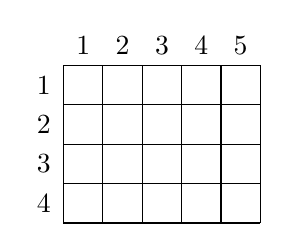
\begin{tikzpicture}[scale=0.5]
\draw (0,0) grid (5,4);

\draw (-0.5,3.5) node{1};
\draw (-0.5,2.5) node{2};
\draw (-0.5,1.5) node{3};
\draw (-0.5,0.5) node{4};
\draw (0.5,4.5) node{1};
\draw (1.5,4.5) node{2};
\draw (2.5,4.5) node{3};
\draw (3.5,4.5) node{4};
\draw (4.5,4.5) node{5};
\end{tikzpicture}
\captionof{figure}{Matrice}
\label{matrice}
\end{center}
\begin{itemize}
\item La \textbf{définition} d'une image de \emph{m} lignes et \emph{n} colonnes est $m×n$. L'image de la figure \ref{matrice} a une définition de $5×4=20~pixels$.
\item La \textbf{résolution} est le nombre de pixels par unité de longueur. On utilise couramment l'unité américaine (le \emph{pouce}). L'écran affiche une résolution de 72ppp (pixels par pouce ).
\item Le format \emph{bitmap (bmp)} est une image matricielle. Les formats \emph{jpeg} (Joint Photographic Experts Group) ou \emph{png} (Portable Network Graphics) sont également des images matricielles \emph{compressées}.
\end{itemize}
\begin{commentprof}
\begin{itemize}
\item en anglais: ppi pixel per inch ou dpi (density per inch)
\item nouveau format webp dvp par google; performance de compression > 30\% par rapport à jpg; pour diminuer quantité de données qui transitent sur le web (60\% d'images)
\end{itemize}
\end{commentprof}
\begin{activite}
Une image quelconque possède 4000 colonnes et 3000 lignes.
\begin{enumerate}
\item Calculer sa définition en pixels. La convertir en mégapixels.
\item Sachant que:
\begin{itemize}
\item la résolution de l'image est 72ppp,
\item $1~pouce = 2,54cm$.
\end{itemize}
Calculer la longueur et la largeur réelle de l'image en centimètres.
\end{enumerate}
\end{activite}
\subsection{Construire une image}
\subsubsection{Noir et blanc}
Chaque pixel ne peut avoir que deux couleurs possibles. Il est possible d'enregistrer l'information sur \emph{1 bit}. Le format \emph{pbm (Portable BitMap)} permet de créer une image simplement.
\begin{activite}
\begin{enumerate}
\item Télécharger le fichier \emph{images-numeriques.zip} sur le site \mbox{\url{https://cviroulaud.github.io}}.
\item Extraire les fichiers du dossier compressé.
\item Ouvrir l'image \emph{cercle.pbm} en double-cliquant sur le fichier.
\end{enumerate}
Nous allons utiliser le logiciel \emph{Notepad++} pour afficher les informations qui composent le fichier. 
\begin{enumerate}[resume]
\item Lancer l'installation du logiciel \emph{Notepad++Portable} dans l'espace personnel ou sur une clé USB.
\item Ouvrir le logiciel \emph{Notepad++Portable} depuis le dossier d'installation.
\item Si le logiciel est en anglais, se rendre dans \emph{Settings/Preferences/General} et changer la langue.
\item Dans \emph{Affichage} cliquer \emph{Retour à la ligne}.
\item Ouvrir à nouveau l'image avec \emph{Notepad++}. La première ligne indique le type de l'image: P1 est une image en noir et blanc.
\item Que représente les informations de la deuxième ligne?
\item Que représente les informations contenues dans ce fichier?
\end{enumerate}
\end{activite}

\subsubsection{Nuances de gris}
Il y a 256 nuances de gris en comptant le noir (0) et le blanc (255). L'information d'un pixel est enregistré sur \emph{1 octet} (soit 8 bits). Le format \emph{pgm (Portable GrayMap)} permet de créer une image en nuance de gris.
\begin{activite}
\begin{enumerate}
\item Ouvrir l'image \emph{nombre.pgm}. Elle semble entièrement noire mais un nombre se cache dans l'image.
\item Ouvrir l'image avec \emph{Notepad++}.
\item Sur la première ligne comment note-t-on une image en nuances de gris?
\item Observer la troisième ligne: combien de nuances de gris peut-on utiliser dans cette image?
\item À l'aide de la fonction \emph{rechercher et remplacer} du bloc-notes, modifier l'image pour faire apparaître le nombre.
\end{enumerate}
\end{activite}
\subsubsection{Image en couleurs}
Pour obtenir une couleur quelconque il faut mélanger une quantité de Rouge, Vert et Bleu. Chaque pixel est représenté par un triplet de nombre entre 0 et 255. Un pixel est enregistré sur \emph{3 octets}. Le format \emph{ppm (Portable PixMap)} permet de créer une image en couleurs.
\begin{activite}
\begin{enumerate}
\item Ouvrir le logiciel \emph{Gimp}.
\item Créer une image carrée de 100 pixels de côté.
\item Enregistrer le fichier (\emph{Fichier/enregistrer}).
\item Créer un rectangle de sélection avec l'outil \emph{sélection} (figure \ref{selection}).
\begin{center}
\centering

\includegraphics[width=1cm]{ressources/selection.png}
\captionof{figure}{Outil de sélection}
\label{selection}
\end{center}
\item Cliquer sur le rectangle supérieur du choix des couleurs (figure \ref{couleur}).
\begin{center}
\centering

\includegraphics[width=1cm]{ressources/couleur.png}
\captionof{figure}{Couleur de premier plan/ d'arrière plan}
\label{couleur}
\end{center}
\item Une fenêtre s'ouvre; choisir une couleur et valider.
\item Dans le menu \emph{Édition}, choisir \emph{Remplir avec la couleur de PP}.
\item Répéter ces opérations pour créer un tableau de couleurs similaires à la figure \ref{tableau}.
\begin{center}
\centering

\includegraphics[width=3cm]{ressources/couleurs.png}
\captionof{figure}{Tableau}
\label{tableau}
\end{center}
\item Exporter le tableau (\emph{Fichier/exporter}) sous le nom \emph{tableau.ppm}. Choisir \emph{ASCII} quand la question est posée.
\item Ouvrir le fichier \emph{tableau.ppm} avec \emph{Notepad++}.
\item Repérer les blocs qui représentent un rectangle et les triplets qui représentent un pixel coloré.
\end{enumerate}
\end{activite}
\section{Métadonnées}
Une image contient de nombreuses informations supplémentaires: les \textbf{métadonnées}. On parle également de données \emph{EXIF} pour \emph{EXchangeable Image File format}.
\begin{activite}
\begin{enumerate}
\item Ouvrir l'image \emph{paysage.jpg} . L'objectif de l'activité est de déterminer la localisation de ce lieu.
\item Ouvrir le site \url{https://www.verexif.com/fr/} .
\item Télécharger la photo et valider.
\item Déterminer la localisation du paysage.
\item Quelles autres informations peuvent être stockées dans les métadonnées?
\end{enumerate}
\end{activite}
\end{Form}
\end{document}